\section{Introduction}

The standard theoretical model for studying molecular electronic systems
consists of \ac{DFT} for obtaining electronic structure, and \ac{NEGF} for
calculating transport properties. In this scheme, electron correlations are
taken into account by inclusion of the exchange-correlation potential $V_{xc}$
in the \ac{DFT} Hamiltonian, and device-lead coupling is included using an
energy-dependent ``Self-Energy'' term $\Sigma(E)$.

Recently, additional use of the GW approximation has become common, in order to
correct for the shifting of quasiparticle levels in the device due to coupling
to, and applied bias on, the leads. It has been shown [cite Neaton, Thygesen]
that this approach corrects significantly the characteristic over-estimation by
\ac{DFT}-based methods of zero-bias conductance and finite bias currents
compared to experimental results.

In a different approach, methods from the field of quantum chemistry, with
which it is possible to incorporate electron correlations to an arbitrary
degree can  used \cite{vici2004} but in those cases, modeling the effect of
coupling to leads is problematic. Including an energy-dependent potential term
in the Hamiltonian is possible in principle, but not feasible in practice.

In earlier work~\cite{henderson}, a method was outlined in which an
energy-dependent self-energy is mapped to an energy-independent
\ac{CAP}, which, when added to the Hamiltonian, can be used
in a many-body treatment of the system. Here, we present a continuation of that
work, applying the method to a chain of atoms with interacting electrons, and
using a complex \ac{CI} scheme for the calculation of electronic structure.
Different levels of correlation are explored by varying the threshold
parameter for \acp{CSF} in the \ac{CI} calculation.

The rest of this paper is organized as follows: in section~\ref{sec:method}, we
cover the methods used in this work, both for constructing the \ac{CAP} and for
solving the resulting complex symmetric many-body problem. In
section~\ref{sec:results} we present and discuss some results of applying the
formalism to a simple atomic chain system. Finally,
section~\ref{sec:conclusions} contains conclusions and further perspectives.


\section{Method}
\label{sec:method}

\subsection{Model System}
\label{subsec:modelsystem}

The system we studied consists of a simple atomic chain with interatomic
separation of 0.28 nm (?), intended to mirror the system studied experimentally
in~\cite{nilius2002science} (See figure~\ref{fig:chaincapdevice}). Two interatomic
spacings are made larger than the others, to delineate a ``device'' between two
leads. This spacing determines the degree to which the device states couple to
the leads, and variation of the spacing allows us to explore different coupling
regimes.

\begin{figure}
	\begin{center}
		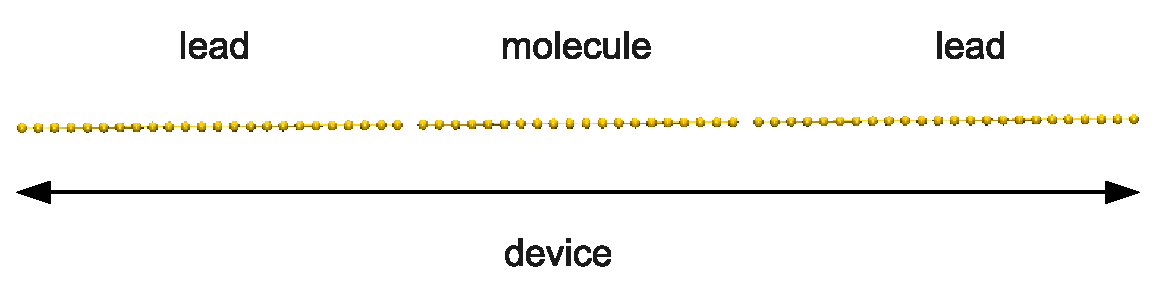
\includegraphics[width=0.9\linewidth]{figures/chaincapdevice}
	\end{center}
	\caption{Model system studied in this work. The device consists of 24
	Gold atoms, while the leads (not fully shown to accentuate the
	device-lead gaps) consist of 20 atoms each.}
	\label{fig:chaincapdevice}
\end{figure}

For comparison purposes, the transmission spectrum of this system was
calculated in the \ac{NEGF} formalism using the TIMES~\cite{times} code. The
objective is to model the peaks of this spectrum with Lorentzian curves for
which the peak location and peak width are extracted from the real and
imaginary parts, respectively, of the complex eigenvalues obtained by
diagonalization of the Hamiltonian which includes a complex symmetric \ac{CAP}.

\subsection{Complex Absorbing Potential}
\label{subsec:CAP}

The procedure for construction of a \ac{CAP} is explained in detail
in~\cite{henderson}; we briefly present the essential points here.

The goal is to introduce a matrix \umm{W} which mimics the effect of coupling
to a semi-infinite lead in a similar way as a complex self-energy
\umm{\Sigma(E)}, but without the energy dependence. In order to achieve this,
we construct \umm{W} such that, when added to the bare Hamiltonian $\um{H}_0$,
it produces the same set of complex eigenvalues and eigenvectors as the
Hamiltonian with \umm{\Sigma(E)} added.

This is achieved by solving the related problem

\begin{subequations}
\begin{align}
	[\um{H} + \lambda \um{\Sigma}(\omega_i^\lambda)] \ket{\psi_i^\lambda}
	&= \omega_i^\lambda \ket{\psi_i^\lambda} \\
	\bra{\varphi_i^\lambda} [\um{H} + \lambda \um{\Sigma}(\omega_i^\lambda)]
	&= \omega_i^\lambda \bra{\varphi_i^\lambda} 
	\label{eq:adiabaticap}
\end{align}
\end{subequations}

for $\lambda$ gradually (adiabatically) increasing from 0 to 1. In this way, we
go from the eigenenergies and eigenstates of $\um{H}_0$ at $\lambda = 0$ to
those of $\um{H}_0 + \um{\Sigma(\omega_i)}$ at $\lambda = 1$.

For the construction of the \ac{CAP}, since our many body code can only deal
with real MO basis sets, we are forced to use the real eigenbasis of \umm{H}
($\um{W}_0$ from \cite{henderson}), defining the \ac{CAP} to be

\begin{equation}
	\um{W} = \um{X}\um{\omega}\um{X}^\dagger - \um{H}_0
	\label{eq:capsdef}
\end{equation}

where \umm{\omega} is a diagonal matrix with the complex value $\omega_i$ as
its $i$th diagonal element.

This projection introduces a small amount of inaccuracy, as will be discussed
later.

\subsection{Complex Monte Carlo Configuration Interaction}

The \ac{CI} calculations were performed using a version of the \ac{MCCI}
program, modified according to the orthogonal projection method outlined
in~\cite{tarantelli_csd} to solve the complex symmetric generalized eigenvalue
problem that results when a \ac{CAP} is introduced into the Hamiltonian. The
\ac{MCCI} program computes energy estimates by an iterative process: starting
from a set of \acp{CSF} (which may be a lone Slater Determinant), a set of
\acp{CSF} are created which consist of single and double excitations from the
starting \ac{CSF} set. These sets are then joined, and the Schr\"odinger
equation is constructed and solved in the corresponding \ac{CI} subspace. Then
follows a pruning step, in which those \acp{CSF} which have a coefficient in
the relevant eigenvector of the Hamiltonian lower (in magnitude) than a given
threshold value $cmin$ are deleted, after which the process is repeated until
convergence is reached.

To explore the effect of electron correlation on the shifts and broadenings, we
ran calculations with different values of the threshold parameter $cmin$.
% Only those \acp{CSF} which excited into or from states localized in the device
% (as opposed to the part of the leads which is included in the device region)
% were considered, since we wanted to explore only excitations of the actual
% device.


\section{Results and Discussion}
\label{sec:results}

\subsection{Single-Particle Picture}
\label{subsec:SingleParticle}

As a validation of the \ac{CAP} approach, we would first like to see whether
the \ac{CAP} as generated according to the description of
section~\ref{subsec:CAP} gives the correct complex single-particle eigenvalues,
i.e. whether the selected self-consistent solutions of the Dyson equation
provide an accurate picture of the resonances in the device region. To this
end, we convert the complex eigenvalues $\omega_i$ of $\um{H} + \um{W}$ to
Lorentzian broadened peaks according to

\begin{equation}
	f(\varepsilon;\omega_i)
	= \frac{\frac{\Gamma}{2}^2}
	       {(\varepsilon - \operatorname{Re}(\omega_i))^2
	       + \frac{\Gamma}{2}^2}
	\label{eq:lobro}
\end{equation}

where $\Gamma = 2 \times \operatorname{Im}(\omega_i)$ is the broadening
associated with the eigenvalue (i.e. the width of the Lorentzian peak), and
compare to a transmission spectrum of the device obtained using the self-energy
in the \ac{NEGF} formalism. Such a comparison is shown in
figure~\ref{fig:lobro-hwevals}, with good agreement between the two. (The
agreement is also obtained outside the plotted range.)

This is a case of weak coupling, as can be seen by the narrowness of the
transmission peaks, and by the fact that they are not significantly shifted
from the real-valued Hartree-Fock single-particle levels, which are indicated
by vertical blue lines in fig.~\ref{fig:lobro-hwevals}. 

\begin{figure}
	\begin{center}
		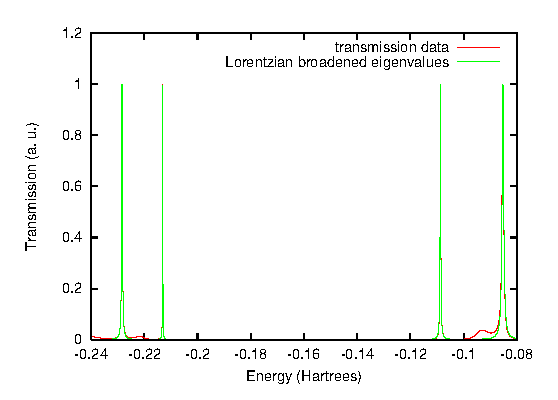
\includegraphics[width=0.9\linewidth]{figures/4evals}
	\end{center}
	\caption{Comparison of transmission data (red) with Lorentzian
	broadened complex eigenvalues of $\um{H}_0 + \um{W}$ (green) for a
	model system as described in section~\ref{subsec:modelsystem}, with
	device-lead gap of 0.45 nm. Transmission data was obtained from
	\ac{NEGF} calculations with the TIMES program~\cite{times}.
        Blue vertical lines indicate the single-particle levels of the device
        in the Hartree-Fock approximation.}
	\label{fig:lobro-hwevals}
\end{figure}

\subsection{Single Determinant}
\label{subsec:SingleDeterminant}

The next step is to pass to the many-body picture, initially representing the
wave function of the $N$ electron system as a single Slater determinant. The
quasiparticle peaks in the transmission spectrum are approximated by taking
differences of many-body energies: $E^N - E^{N-1}$ yields the \ac{HOMO}, while
likewise $E^{N+1} - E^N$ yields the \ac{LUMO} (other quasiparticle levels can be
obtained by taking differences of excited many-body energies). The peaks for
the \ac{HOMO} and \ac{LUMO} of the system obtained in this way are plotted in figure

\subsection{Single Excitations}
\label{subsec:singles}

The next step is to include, for each state, the reference determinant plus all
its single excitations. By Thouless' theorem~\cite{Thouless}, the wave function
obtained in this way would still be describable as a single determinant (and
thus, by definition, contain no correlation), but by adding degrees of freedom
to the system, a degree of self-consistency is attained. The results for the
\ac{HOMO} and \ac{LUMO} quasiparticle levels are plotted in
figure~\ref{fig:cipeaks}.

\begin{figure}
	\begin{center}
		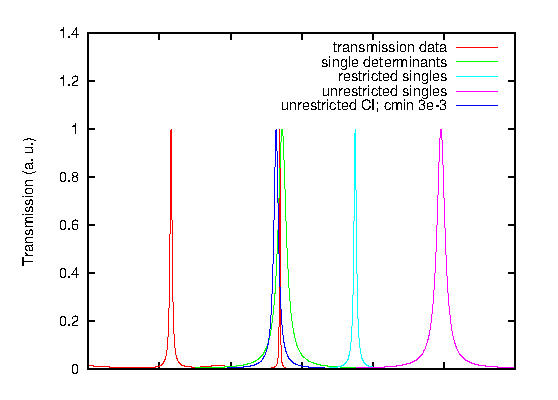
\includegraphics[width=0.9\linewidth]{figures/ci_4.5A_homo.eps}
	\end{center}
	\caption{}
	\label{fig:cipeaks}
\end{figure}

Finally, we start adding correlation:

\begin{figure}
	\begin{center}
		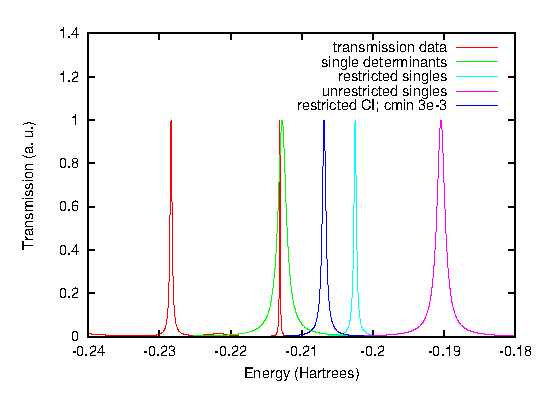
\includegraphics[width=0.9\linewidth]{figures/cidevice_4.5A_homo.eps}
	\end{center}
	\caption{}
	\label{fig:cipeaks-device}
\end{figure}

\section{Conclusions}
\label{sec:conclusions}

